\chapter[Indicatori VAN-WACC]{Indicatori VAN-WACC}
\section[VAN]{VAN}
	\begin{equation}
	\label{eq:van}
	\begin{split}
 		w = \sum_{k=0}^n \frac{C_k}{(1+r)^k}
	\end{split}
	\end{equation}
	ci possiamo, quindi, calcolare il valore del \ac{TIR} corrispondente. Per definizione il \ac{TIR} è pari a:
	\begin{equation}
	\label{eq:tir}
	\begin{split}
 		\sum_{k=0}^n \frac{C_k}{(1+i)^k} = 0
	\end{split}
	\end{equation}	 

	L'andamento del \ac{VAN} in funzione dei flussi mensili è rappresentabile dalla seguente formula:	
	\begin{eqnarray}
	\label{eq:andamento_van_flussi}
 		y(x) & = & 10,7528 \cdot ( x - 60131,27 ) - 56170,20		\nonumber \\
 			 & = & 10,7528 \cdot x - 702749,72
	\end{eqnarray}

 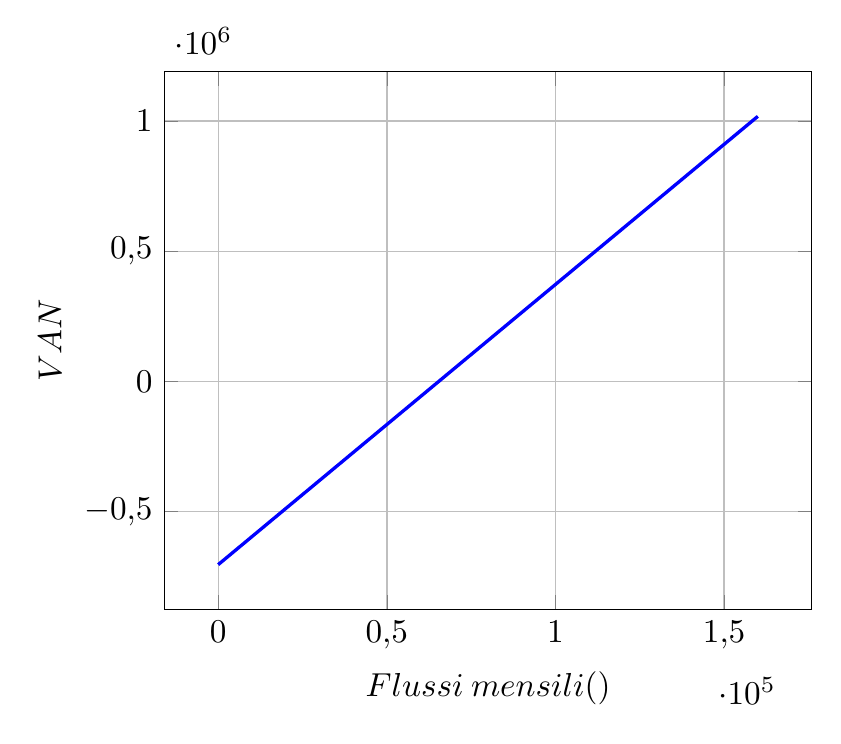
\begin{tikzpicture}[scale=1.2]
 \pgfkeys {
			/pgf/number format/.cd,
			set decimal separator={,{\!}},
			set thousands separator={}}
	\begin{axis}[ xlabel=$Flussi\: mensili (\mbox{\euro})$, 
				   ylabel=$VAN$, 
				   grid=major ]
		
		\addplot[domain=0:160000, color=blue, line width=1pt]{10.7528 * x - 702749.72};
		
	\end{axis}
\end{tikzpicture}

Un punto importante della funzione \ref{eq:andamento_van_flussi} è quello per cui il $ VAN = 0 $, ovvero:

	\begin{equation}
	\label{eq:van_zero}
	\begin{split}
 		y(x) = 0
 	\end{split}
	\end{equation}

Il valore $x$ corrispondente è pari alla quantità di flussi di cassa mensili minimi che dovremmo avere per rendere il progetto remunerativo. Il valore del flusso di cassa per cui è soddisfatta \ref{eq:van_zero} è, ponendo:
			
	\begin{equation}
	\label{eq:van_pareggio_1}
	\begin{split}
 		10,7528 \cdot x - 702749,72 = 0	
 	\end{split}
	\end{equation}			

pari a (in \euro):
			
	\begin{eqnarray}
	\label{eq:van_pareggio_2}
		x & = & \frac{702749,72	}{10,7528}	 	\nonumber \\[1.5ex] 
		  & = & 65355,04
	\end{eqnarray}

\subsection[Break-even period]{Break-even period}
	Si analizza, infine, il \textbf{punto di pareggio}, ovvero la quantità di chiamate necessarie per avere un fatturato tale da ricoprire l'investimento iniziale, in modo tale da chiudere il periodo di riferimento senza perdite né profitti.

Il \textbf{break even period} (periodo di pareggio), ovvero il periodo di tempo necessario per il recupero dell'esborso iniziale è quindi pari a:   	

\subsection[Caso di Studio]{Caso di Studio}


\subsubsection[Caso Teorico]{Caso Teorico}

%
%	Tabella relativa al caso teorico in cui non ci siano malati durante un anno
%
\begin{savenotes}
\begin{table}[htb]
\centering
 \caption{Variazione VAN (Caso Teorico)}
 \begin{tabular}{p{4cm}D{,}{,}{5.2}D{,}{,}{5.2}D{,}{,}{5.2}D{,}{,}{7.4}}
 \toprule
 	& \multicolumn{1}{c}{Flusso di cassa mensile (\euro)} & \multicolumn{1}{c}{Contratti Mensili } &\multicolumn{1}{c}{\textbf{VAN}}&\multicolumn{1}{c}{\textbf{ \% Contratti}} \\
 \midrule	
 	\makebox[4cm][r]{Pareggio} & 65355,07 & 939,18 & 0,00 & 0,1154\\ 
	\makebox[4cm][r]{Ottimo} & 553419,36 & 8138,52 & 5248057,65 & 1,0000\\
	\makebox[4cm][r]{Caso di Studio 20,0 \%} & 110683,87 & 1627,70 & 487411,50 & 0,2000\\
	\makebox[4cm][r]{Caso di Studio 15,0 \%} & 83012,90 & 1220,78 & 189871,11 & 0,1500 \\
	\makebox[4cm][r]{Caso di Studio 12,5 \%} & 69177,42 & 1017,32 & 41100,92 & 0,1250 \\
 \bottomrule
 \end{tabular} 
\end{table}
\end{savenotes}


\subsubsection[Caso UNIFORME]{Caso UNIFORME}

%
%	Tabella relativa al caso in cui il numero di malati si distribuisce in maniera uniforme durante l'anno
%
\begin{savenotes}
\begin{table}[htb]
\centering
 \caption{Variazione VAN (Malati distribuiti uniformemente)}
 \begin{tabular}{p{4cm}D{,}{,}{5.2}D{,}{,}{5.2}D{,}{,}{5.2}D{,}{,}{7.4}}
 \toprule
 	& \multicolumn{1}{c}{Flusso di cassa mensile (\euro)} & \multicolumn{1}{c}{Contratti Mensili } &\multicolumn{1}{c}{\textbf{VAN}}&\multicolumn{1}{c}{\textbf{ \% Contratti}} \\
 \midrule	 
	\makebox[4cm][r]{Ottimo} & 615888,00 & 7698,60 & 4926392,37 & 1,0000\\
	\makebox[4cm][r]{Caso di Studio 15,0 \%} & 92406,24 & 1155,078 & 141831,90 & 0,1500 \\
 \bottomrule
 \end{tabular} 
\end{table}
\end{savenotes}

\subsubsection[Caso OTTIMO]{Caso OTTIMO} 

%
%	Tabella relativa al caso in cui il numero di malati si concentra nel mese di Dicembre
%
\begin{savenotes}
\begin{table}[htb]
\centering
 \caption{Variazione VAN (Malati nel mese di Dicembre)}
 \begin{tabular}{p{4cm}D{,}{,}{5.2}D{,}{,}{5.2}D{,}{,}{5.2}}
 \toprule
 	& \multicolumn{1}{c}{Flusso di cassa mensile (\euro)} & \multicolumn{1}{c}{Contratti Mensili } &\multicolumn{1}{c}{\textbf{VAN}} \\
 \midrule	 
	\makebox[4cm][r]{Caso di Studio 15,0 \%} & 39592,80 & 494,91 & 150010,00 \\
 \bottomrule
 \end{tabular} 
\end{table}
\end{savenotes}

\subsubsection[Caso PEGGIORE]{Caso PEGGIORE}

%
%	Tabella relativa al caso in cui il numero di malati si concentra nel mese di Gennaio
%
\begin{savenotes}
\begin{table}[htb]
\centering
 \caption{Variazione VAN (Malati nel mese di Gennaio)}
 \begin{tabular}{p{4cm}D{,}{,}{5.2}D{,}{,}{5.2}D{,}{,}{5.2}}
 \toprule
 	& \multicolumn{1}{c}{Flusso di cassa mensile (\euro)} & \multicolumn{1}{c}{Contratti Mensili } &\multicolumn{1}{c}{\textbf{VAN}} \\
 \midrule	 
	\makebox[4cm][r]{Caso di Studio 15,0 \%} & 29034,40 & 362,93 & 132972,00 \\
 \bottomrule
 \end{tabular} 
\end{table}
\end{savenotes}



\section[WACC]{WACC}
	\begin{equation}
	\label{eq:wacc}
	\begin{split}
		WACC = \frac{D}{D+E} \cdot K_d + \frac{E}{D+E} \cdot K_e 
	\end{split}
	\end{equation}
	La formula \ref{eq:wacc}, però non tiene conto della quota di imposte che gravano sulla quota da restituire (cioè sul valore di \textbf{D}). \newline Se definiamo con \textbf{t}, il valore della quota di imposte che gravano su \textbf{D} ( nel nostro caso $ t = 0,15 $ ), allora la \ref{eq:wacc} diventa:
	\begin{equation}
	\label{eq:wacc_tax}
	\begin{split}
		WACC = \frac{D}{D+E} \cdot K_d \cdot ( 1 - t ) + \frac{E}{D+E} \cdot K_e 
	\end{split}
	\end{equation}	
	Il nostro caso di studio prevedeva di richiedere un finanziamento di \euro 30000,00 presso la \textbf{\ac{Fibank Albania}} in modo tale da essere in grado di fronteggiare le spese di installazione dei vari impianti in quanto la quota iniziale a disposizione dei soci fondatori non era sufficiente.
\newline
La \textbf{\ac{Fibank Albania}} prevede, in particolare una quota di interesse pari al 4,4 \% della quota del finanziamento, quindi in questo caso dovremmo restituire circa (in \euro):
	\begin{equation}
	\label{eq:interessi_fibank}
	\begin{split}
		quota interessi = 0,044 \cdot 30000 = 1320 
	\end{split}
	\end{equation}	
Il nostro valore del \ac{WACC}, quindi, sarà pari a:
	\begin{equation}
	\label{eq:wacc_tax_value}
	\begin{split}
		WACC = \frac{30000}{65000} \cdot 0,044 \cdot ( 1 - 0,15 ) = 0,01726 
	\end{split}
	\end{equation}